% !TeX root = ../thuthesis-example.tex


\chapter{基础理论介绍}
\label{chap:background}

\section{计算机视觉基础} % 图

\subsection{卷积神经网络}
卷积神经网络(CNN)是深度学习中处理网格结构数据的重要模型。它利用局部感受野、参数共享和降采样机制来提取图像特征。CNN主要由三类层次构成:卷积层负责特征提取,池化层实现特征压缩,全连接层完成特征映射。这种结构设计使CNN在计算机视觉领域获得了广泛应用。
% 卷积神经网络的一个重要特点是其层次化的特征学习能力。浅层网络主要学习边缘、纹理等低级视觉特征,随着网络层数加深,逐渐过渡到形状、部件等中级特征,最终学习到语义级的高级特征表示。这种层次化的特征提取机制使得CNN在图像分类、目标检测等视觉任务上取得了突破性进展。

\subsection{3D卷积神经网络}
相比于处理单帧图像的2D CNN,3D CNN在时间维度上引入了额外的卷积操作,能够同时对视频数据的空间和时间特征进行建模。如图~\ref{fig:3dcnn}所示,3D卷积层使用三维卷积核在输入体积上进行滑动,提取时空联合特征。
这种结构设计让3DCNN可以有效提取视频中的时序动态特征,为视频分析和理解提供了重要的技术支持。
在3D CNN的发展历程中,C3D~\cite{tran2015c3d}是一个重要的里程碑。该模型首次将3D卷积应用于大规模视频分类任务,通过端到端的训练方式学习视频的时空特征表示。
% 建议在这里插入一张3D CNN结构示意图
\begin{figure}[htbp]
    \centering
    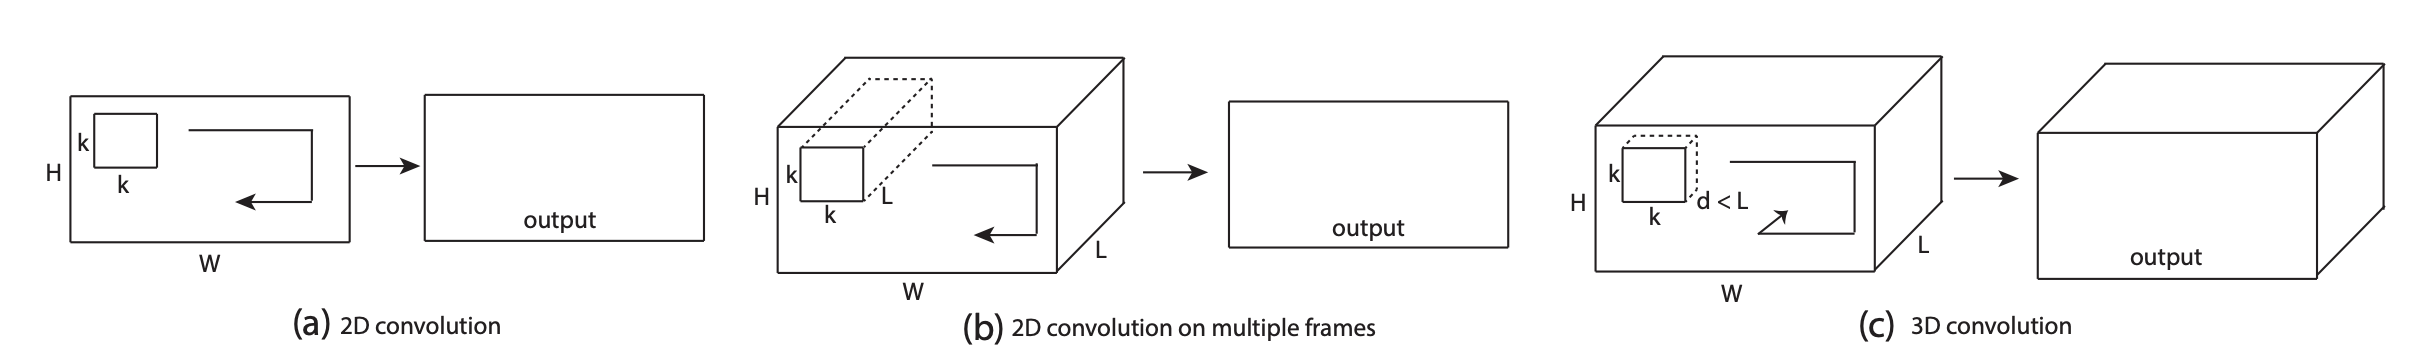
\includegraphics[width=\linewidth]{3dcnn.png}
    \caption{2D 和 3D 卷积示意图~\cite{tran2015c3d}。2D 卷积在图像或视频帧上运算得到特征图,而 3D 卷积可在视频序列上同时提取时空特征。}
    \label{fig:3dcnn}
\end{figure}

\subsection{视觉变换器}
近年来,Transformer被广泛应用于计算机视觉领域。
视觉变换器(Vision Transformer,ViT)是这一探索的代表性成果。不同于CNN基于局部感受野的特征提取方式,ViT将输入图像分割成固定大小的图像块(patches),并将这些图像块序列化后输入Transformer进行处理。通过自注意力机制,ViT能够建模图像块之间的全局依赖关系,为视觉特征提取提供了新的范式。

鉴于视觉 Transformer 在图像领域的成功,一些工作将其拓展到视频领域,提出了视频变换器(Video Transformer)。
典型的 Video Transformer 结构包括 时空分离(Spatiotemporal Separated) 和 时空联合(Joint Spatiotemporal) 两种策略。前者如 TimeSformer \cite{bertasius2021space},通过独立的时间和空间注意力进行计算,减少计算复杂度;后者如 ViViT \cite{arnab2021vivit},直接在 3D 令牌(Token)上施加全局注意力,以获得更强的时空建模能力。视频变换器在动作识别、视频理解等任务上已经展现出强大的性能。

% 建议在这里插入一张Video Transformer结构示意图
\begin{figure}[htbp]
    \centering
    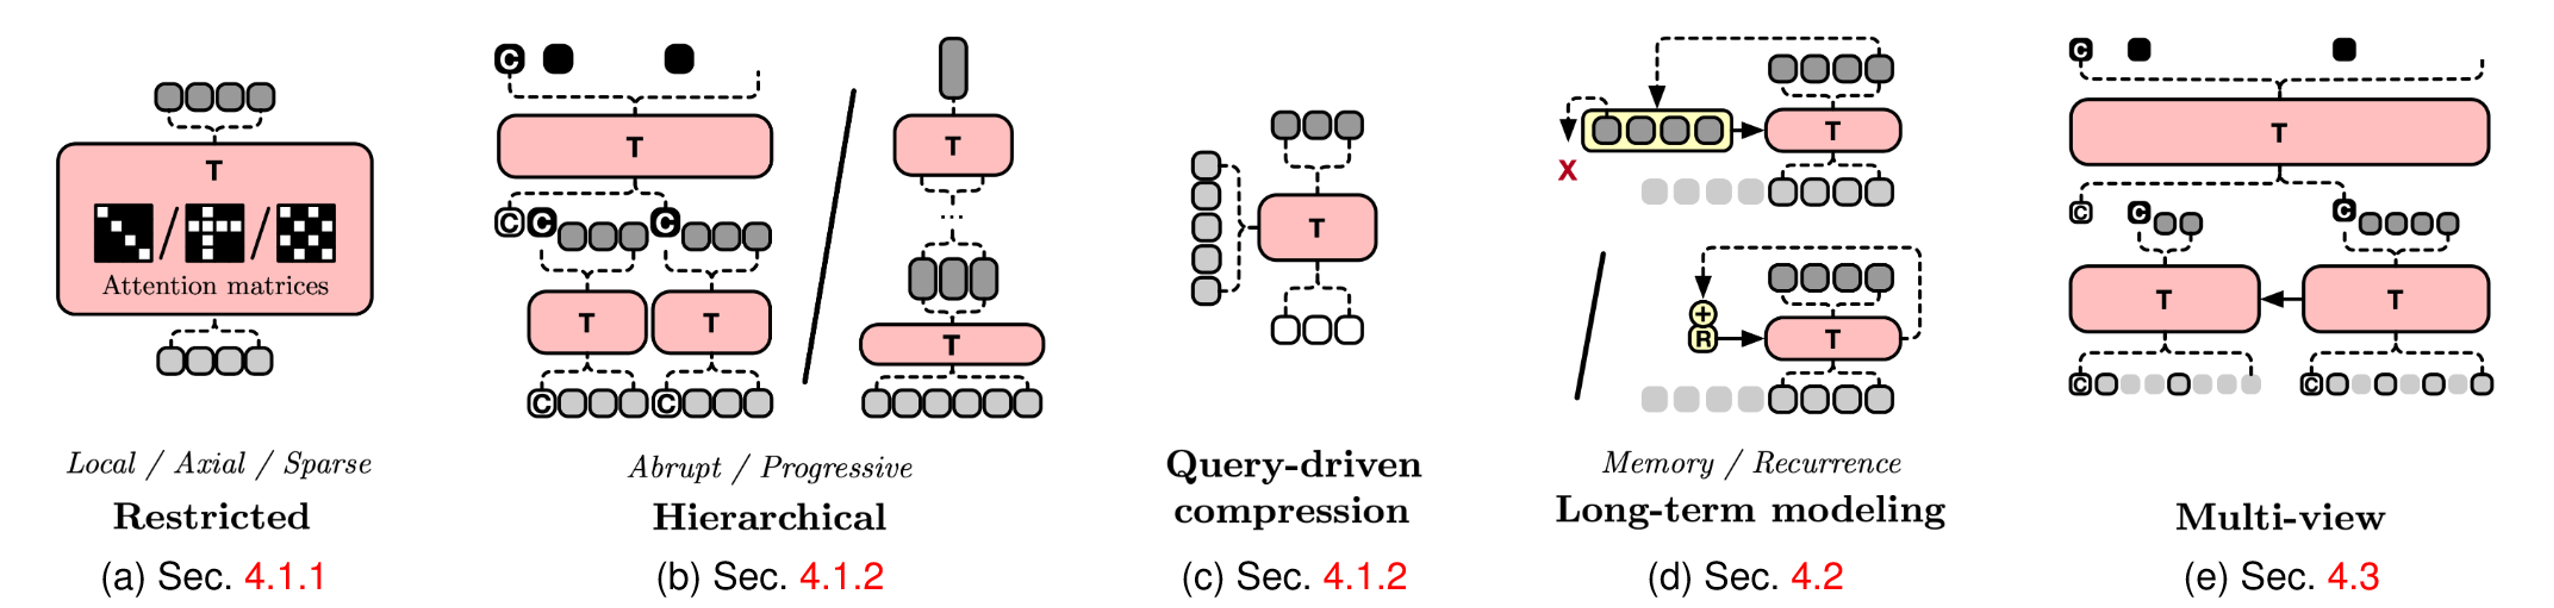
\includegraphics[width=\linewidth]{vt.png}
    \caption{Video Transformer 不同设计选择的可视化~\cite{selva2023video}。数据标记采用浅灰色(如果使用标记则采用黑色描边),而增强标记采用深灰色;白色标记是初始化的可学习标记;[CLS] 标记用“C”表示(增强后填充黑色)。从侧面流入变压器(T)的数据用于交叉注意。}
    \label{fig:vt}
\end{figure}

\section{生成模型基础}

\subsection{变分自编码器}

变分自编码器(VAE)\cite{kingma2013vae} 是一类通过概率建模实现数据生成的深度学习模型。
与传统自编码器不同,VAE 的核心思想是对潜在变量进行概率建模,学习数据的概率分布,而不是直接学习数据到数据的映射。这种基于概率的建模方式使得VAE能够生成多样化的样本,并且具有良好的插值性质。

VAE 假设观测数据由某个潜在变量生成,其生成过程可表示为 $p_{\theta}(\mathbf{x} \mid \mathbf{z})$,其中 $\mathbf{z}$ 服从某一先验分布(通常为标准正态分布)。然而,直接计算后验分布 $p_{\theta}(\mathbf{z} \mid \mathbf{x})$ 通常是不可行的,因此 VAE 采用变分推断,引入一个近似分布 $q_{\phi}(\mathbf{z} \mid \mathbf{x})$ 来进行估计。
模型的优化目标是最大化数据的对数似然,由于难以直接计算,通常转而最大化其证据下界(ELBO):
\begin{equation}
    \log p_{\theta}(\mathbf{x}) \geq \mathbb{E}_{q_{\phi}(\mathbf{z} \mid \mathbf{x})} \left[ \log p_{\theta}(\mathbf{x} \mid \mathbf{z}) \right] - D_{\mathrm{KL}} \left( q_{\phi}(\mathbf{z} \mid \mathbf{x}) \parallel p(\mathbf{z}) \right).
\end{equation}
其中,第一项鼓励模型在给定 $\mathbf{z}$ 的情况下能够准确重构数据,第二项则约束潜在变量的分布,使其接近先验分布,以保证生成的合理性。

在实际实现中,VAE 采用神经网络参数化编码器和解码器,其中编码器将输入数据映射为潜在变量的均值和方差,并通过重参数化技巧 $\mathbf{z} = \boldsymbol{\mu} + \boldsymbol{\sigma} \odot \boldsymbol{\epsilon}$(其中 $\boldsymbol{\epsilon} \sim \mathcal{N}(\mathbf{0}, \mathbf{I})$)实现可微分的采样。最终,通过梯度优化训练,使 VAE 既能够进行数据重构,又能生成高质量的新样本。

% 在训练过程中,VAE通过最大化数据的边际似然来优化模型参数。为了使优化过程可行,VAE引入了变分推断的思想,使用神经网络来近似后验分布。模型的训练目标包括重构误差和KL散度两部分,这种设计既保证了重构质量,又能够约束隐变量空间的结构。在本文手势生成任务中,VAE用于学习手势动作的低维表示,为后续的条件生成提供基础。

\subsection{扩散模型}
扩散模型(Diffusion Model)~\cite{ho2020ddpm} 是一类生成模型,通过逐步去噪的方式学习从噪声分布到数据分布的映射。该模型由前向(扩散)过程和反向(去噪)过程组成,其中前向过程逐步向数据添加噪声,而反向过程学习从噪声中逐步恢复数据分布,实现样本生成。
扩散模型的一个重要优势是其生成结果多样,生成质量高。通过精心设计的噪声调度,模型能够逐步学习数据分布的不同尺度特征。

% 建议在这里插入扩散模型原理示意图
% \begin{figure}[htbp]
%     \centering
%     % \includegraphics[width=0.8\linewidth]{diffusion.pdf}
%     \caption{扩散模型的前向和反向过程示意图}
%     \label{fig:diffusion}
% \end{figure}

\subsubsection{扩散模型的前向与反向过程}
\textbf{前向过程}通过在 $T$ 个时间步内逐步向数据样本 $\mathbf{x}_0 \sim q(\mathbf{x}_0)$ 添加高斯噪声,形成数据序列 $\{\mathbf{x}_t\}_{t=1}^{T}$,其定义如下:
\begin{equation}
    q(\mathbf{x}_t \mid \mathbf{x}_{t-1}) = \mathcal{N}(\mathbf{x}_t; \sqrt{1 - \beta_t} \mathbf{x}_{t-1}, \beta_t \mathbf{I}),
\end{equation}
其中,$\beta_t \in (0,1)$ 为控制噪声水平的方差调度参数。通过重参数化技巧,该分布可直接表示为 $\mathbf{x}_0$ 的函数:
\begin{equation}
    q(\mathbf{x}_t \mid \mathbf{x}_0) = \mathcal{N}(\mathbf{x}_t; \sqrt{\bar{\alpha}_t} \mathbf{x}_0, (1 - \bar{\alpha}_t) \mathbf{I}),
\end{equation}
其中 $\bar{\alpha}_t = \prod_{i=1}^{t} (1 - \beta_i)$。此公式允许从任意中间时间步高效采样。

\textbf{反向过程}旨在建模后验分布 $q(\mathbf{x}_{t-1} \mid \mathbf{x}_t)$,但该分布通常难以直接求解。为此,使用可学习的神经网络 $p_{\theta}$ 进行近似:
\begin{equation}
    p_{\theta}(\mathbf{x}_{t-1} \mid \mathbf{x}_t) = \mathcal{N}(\mathbf{x}_{t-1}; \boldsymbol{\mu}_{\theta}(\mathbf{x}_t, t), \Sigma_{\theta}(\mathbf{x}_t, t)).
\end{equation}
在大多数实现中,协方差 $\Sigma_{\theta}(\mathbf{x}_t, t)$ 可以固定或学习,而均值 $\boldsymbol{\mu}_{\theta}(\mathbf{x}_t, t)$ 通常由神经网络建模。

训练过程中,模型学习预测加入的噪声 $\boldsymbol{\epsilon}$,训练目标是最小化重建误差:
\begin{equation}
    \mathcal{L} = \mathbb{E}_{t,\mathbf{x}_0,\boldsymbol{\epsilon}}[\|\boldsymbol{\epsilon} - \boldsymbol{\epsilon}_\theta(\sqrt{\bar{\alpha}_t}\mathbf{x}_0 + \sqrt{1-\bar{\alpha}_t}\boldsymbol{\epsilon},t)\|_2^2].
\end{equation}
在推理阶段,模型通过从标准高斯分布 $\mathbf{x}_T \sim \mathcal{N}(\mathbf{0}, \mathbf{I})$ 逐步去噪,最终生成符合数据分布的样本。
通过这种设计,扩散模型能够在保证生成质量的同时,实现稳定的训练过程。


\subsubsection{条件扩散模型}
扩散模型通过在去噪过程中引入条件信息,可以实现对生成过程的精确控制。目前条件控制生成主要有两种范式:基于分类器引导的事后修改(Classifier-Guidance)~\cite{dhariwal2021diffusion}和无分类器引导的事前训练(Classifier-Free)~\cite{ho2022classifier}。

分类器引导方法(Classifier-Guidance)首先训练一个无条件扩散模型,然后在推理阶段通过额外的分类器进行条件控制。
这种方法的优点是训练成本较低,可以复用已有的预训练模型;但其缺点是推理计算开销大,且对生成结果的细节控制能力有限。此外,分类器的质量也会直接影响生成效果。

无分类器引导的方法(Classifier-Free-Guidance)则直接在扩散模型的训练过程中加入条件信号,使模型能够在生成过程中自然地融入条件信息,而无需依赖显式的分类器。这种方法能够实现更精细的条件控制,生成质量也更有保障。但其主要缺点是需要较大的训练开销,对计算资源和训练数据的要求较高。
% 在实际应用中,需要根据具体场景的资源约束和性能需求来选择合适的条件控制策略。

